
\section{Fixed-Parameter Intractability}

We will start by giving some intractability results and show that \sdom is \WTWOhs-hard on \textit{bipartite graphs} by a parameterized reduction from \dom on bipartite graphs, which is known to be \WTWOhs \cite{Raman2008}.

\begin{figure}[ht]
    \label{fig:bipartiteConstruction}
    \begin{equation*}
        \tikzfig{fig/tikz/wbipartite}
    \end{equation*}
\caption[Construction bipartite]{\textit{Reducing to a bipartite $G'$ from the bipartite graph $K_{m,n}$ by duplicating all vertices and adding exactly two forced witnesses.}}
\end{figure}

\begin{theorem}
    \sdom is \WTWOhs-hard when restricted to bipartite graphs.
\end{theorem}

\begin{proof}
    We reduce from \dom and consider only $X, Y \neq \emptyset$.
    Given a bipartite $G = ( X \cup Y, E)$, we construct a bipartite graph $G' = (\{X' \cup Y'\},E')$:
    \begin{enumerate}[topsep=0pt,itemsep=0ex,partopsep=1ex,parsep=1ex]
        \item For each $x_i \in X$, we add a new vertex $a_i \in A$  and an edge $\{x_i, a_i\}$ in between. 
        \item For each $y_j \in Y$, we add a new vertex $b_j \in B$ and an edge $\{y_j, b_j\}$ in between.
        \item We add two $P_2$'s with the vertices $u_j,d_j$ and connect their ends to all $a_i$ (resp. $b_i$).
    \end{enumerate}

    $G'$ is bipartite because $A$ and $B$ form an independent set on $G'$ that can be cross-wise attached to $X$ and $Y$. 
    $X' = X \cup \{u_2,d_1\} \cup B$ and $Y' = X \cup \{u_1,d_2\} \cup A$ form the partitions of the new bipartite $G'$.
    It is left to show that $G$ has a ds $D$ of size $k$ if and only if $G'$ has a sds $D'$ of size $k' = k + 2$.
 
    First, assume a ds $D$ in $G$ of size $k$. 
    We know that $D' = D\cup \{d_1,d_2\}$ is an sds in $G'$ of size $k' = k + 2$, because $d_1$ dominates $u_1$ and all $a_i \in A$; $d_2$ dominates $u_2$ and all $b_i \in B$. 
    The same vertices dominate the rest as they were in $G$, but now they all have either $d_1$ or $d_2$ as a witness.
    Therefore,  $\forall v \in (D \cap X) \cup (D \cap Y): (d(v, d_1) = 2 \vee d(v, d_2)=2)$.

    Contrary, assume an sds $D'$ in $G'$ with size $k'$. 
    Wlog, assume that $d_1, d_2 \in D$ and $u_1,u_2 \notin D$, because choosing $d_i$ is preferred to $u_i$.
    By technical assumption $X, Y \neq \emptyset$, $u_i$ can not be a witness for $d_i$.
    If $a_i,b_i \in D'$ we replace it with $x_i$ and $y_i$ preserving the size $D$.
    A $a_i \in A$ can only be used to dominate their neighboring $x_i$ ($b_i \in B$ for $y_i$), because $\abs{N(a_i)} = 2$ and $d_1,d_2\in D'$.

    As $d_1$ and $d_2$ suffice to provide a witness for every vertex in the graph, this operation is sound.
    Hence, $D = D' \setminus \{ d_1,d_2\}$ gives a ds in $G$ of size $ k = k' + 2$.

    As $G'$ can be constructed in linear time and $k$ does not depend on the input size, this reduction is an fpt reduction.  
    Because \dom is \WTWOhs-hard on bipartite graphs \cite[Th. 1]{Raman2008}, we conclude that \sdom is $w[2]$-hard as well.
\end{proof}

Next, we will prove intractability for \textit{split} and \textit{chordal} graphs.

\begin{theorem}
    \sdom is \WONEhs-hard when restricted to \textit{split} and \textit{chordal} graphs.
\end{theorem}

\begin{proof}
    We reduce from \dom on \textit{split} graphs which is visualized in \cref{fig:splitgraph}.
    Given a split graph $G = \{(K \cup I), E\}$, we transform it to a split graph $G'$ by adding two vertices $d$ and $u$ and edges $\{d,u\} \cup \{d, k_i\}$ for all $k_i \in K$. 
    The vertex $d$ increases the size of the clique $K$ by one, and $u$ fits into the independent set $I$.
    Therefore, $G'$ is split, too. 
    It is left to show that $G$ has a ds of size $k$ if and only if $G'$ has an sds of size $k' = k + 1$.
    
    Assume any ds $D$ of size $k$ in $G$. 
    Setting $D' = D \cup \{d\}$ gives an sds in $G'$ of size $k+1$.

    Contrarily, assume an sds $D'$ of size $k$ in $G'$.
    If $D \cap I \neq \emptyset$, we flip these to their neighbor in $K$, preserving the dominating set. 
    $d \in D'$ is only used in $G'$ for dominating $u$ and can be ignored in $G$.
    Therefore letting $D = D' \setminus \{d\}$ gives a valid ds in $G$ of size $ k-1$.
    The claim follows because \dom is \WTWOhs-hard on \textit{split} graphs \cite{Raman2008}.

\end{proof}

\begin{figure}[ht]
    \label{fig:splitgraph}
    \begin{equation*}
        \tikzfig{fig/tikz/split}
    \end{equation*}
\caption[Constructing split graph]{\textit{Constructing a split graph $G'$ by increasing the size of the complete graph by one with a new vertex $d$ and adding one additional pendant $u$. The clique $K$ is highlighted in \textbf{\textcolor{TUMBlue}{blue}}}}
\end{figure}

% \subsection{\hmath  $W[2]$-hard on s Chordal IDK}
% 
% % TODO: Fix everything here.
% Although the previous result implies $w[2]$-hardness for chordal graphs, we found another reduction from \dom on chordal graphs.
% 
% 
% We will introduce the notion of elimination ordering.
% 
% \begin{definition}[{\cite[Theorem 1]{Rose1960}}]
%     In a graph \G with n vertices, a vertex is called \textbf{simplicial} if and only if the subgraph of $G$ induced by the vertex set $\{v\} \cup N(v)$ is a complete graph.
% 
%     $G$  is said to have a \textbf{perfect eliminiation ordering} if and only if there is an ordering $(v_1, ... v_n)$ of the vertices, such that each $v_i$ is simplicial in the subgraph induced by the vertices $v_1,...,v_i\{\}$
% \end{definition}
% 
% The following lemma shows that 
% 
% \begin{lemma}[{\cite[Theorem 1]{Rose1960}}]
%         A graph \G is chordal if and only if $G$ has a perfect elimination ordering.
% \end{lemma}
% 
% \begin{theorem}
%     \sdom restricted to chordal graphs is $\omega[2]$-hard.
% \end{theorem}
% 
% \begin{figure}[!ht]
%     \label{fig:chordalReduction}
%     \begin{equation*}
%         \tikzfig{fig/tikz/chordal-reduction}
%     \end{equation*}
% \caption[Constructing a chordal $G'$]{\textit{Constructing a chordal $G'$ from the chordal graph $P_4$ by adding a $K_5$, connecting its vertices pairwise to $G$. Adding the (blue) auxiliary vertices are necessary to preserve chordality.}}
% \end{figure}
% 
% \begin{proof}
%     
%     We will give a reduction from \dom on chordal graphs.
%     Given \G with vertex set $V = \{v_1,...v_n\} $, we construct a chordal graph $G'$ as described below:
%     \begin{enumerate}
%         \item Add one complete graph $K_{n+1}$ consisting of the vertices \{$k_1,...,k_n,u\}$ and an edge $\{v_i, k_i\}$ to each vertex $v_i \in V$ of $G$. One vertex of the complete subgraph is not connected to any $v \in V$. Denote it as $u$.
%         \item Add one additional vertex $t$ and connect it with $u$ vie the edge $\{u,t\}$.
%         \item For all vertices $v_i \in V$ in $G$, add a new edge $\{n, k_i\}$ for all neighbors $n \in N(v_i)$.
%     \end{enumerate}
% 
%     An example reduction on the graph $P_4$ is shown in  \cref{fig:chordalReduction}.
% 
%     \begin{corollary}\label{cliqueNeighbor}
%        $N(v_i) \in G$ forms a clique iff $N(v_i)$ forms a clique in $G'$
%     \end{corollary}
% 
%     \begin{subproof}
% 
% \begin{figure}[th]
%     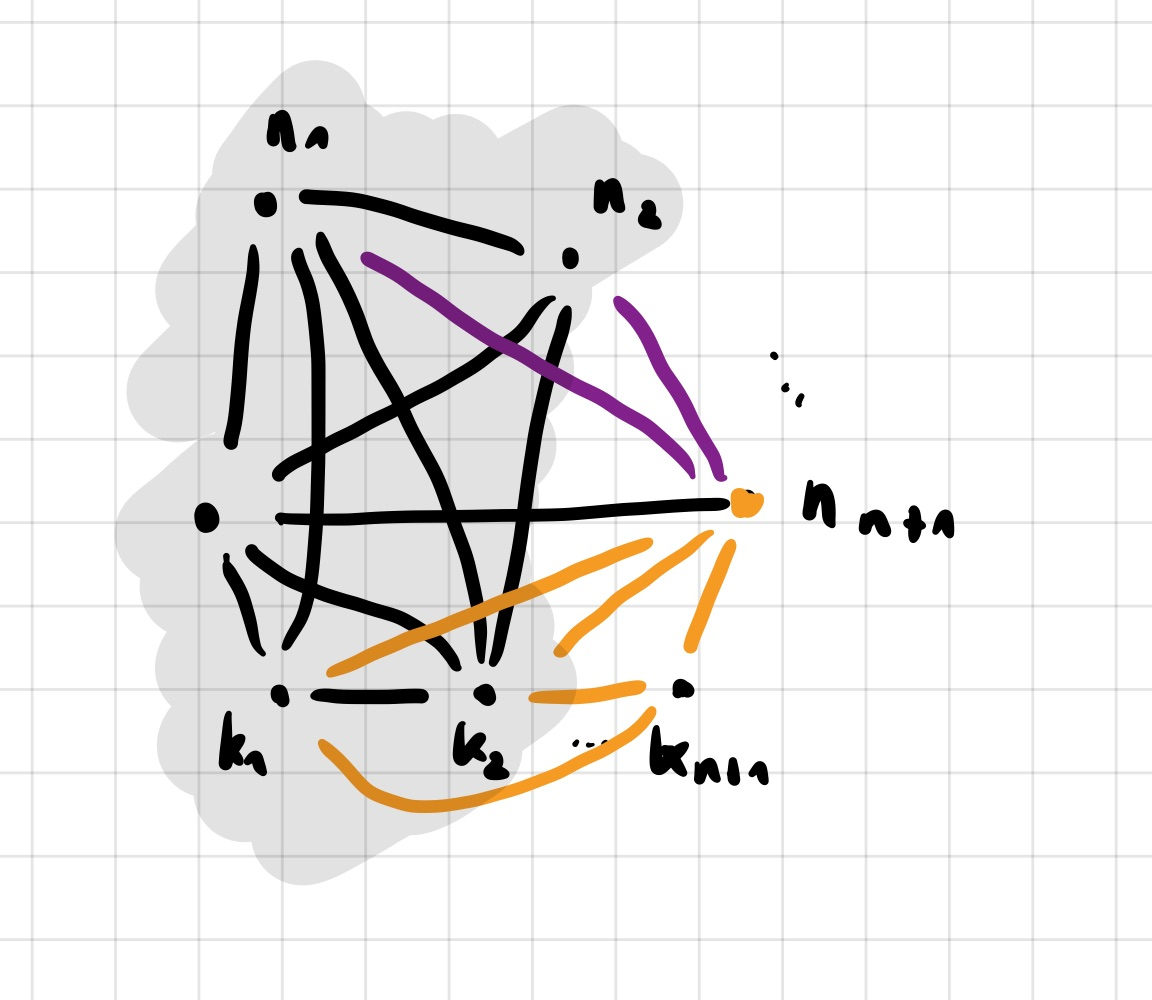
\includegraphics[scale=0.15]{pages/img/induction-step.jpg}
%     \centering
%     \caption{Induction Step}
%     \label{fig:induction-step}
% \end{figure}
% 
%         Asuming that $N(v_i)$ forms a clique in G, we show that it also forms a clique in G' by induction over the number of neighbors $z = abs(N(v_i))$ in G.
% 
%         \begin{itemize}
%             \item $z = 0$: Holds trivially as we do not have a neighbor in G and in G' the connected $k_i$ forms a $P_1$, hence a clique.
%             \item $z = z + 1$: 
% 
%             By IH, we already know that all neighbors $n_1,...,n_z$ form a clique together with their vertices in $k_{i}$. As $k_{z+1}, v_{z+1} \in N(v_i)$ now also in G', we show that $N(v_i)$ still forms clique in G'.
% 
%             Let $k_i$ be the vertex that was connected with $n_i$ during step 1. All we have to show is that $v_{z+1}$ and $k_{z+1}$ extend our previous clique, hence are fully connected with $N(v_i)$.
%             
%             $v_{z+1}$ connects to $N(v_i)$ in G by assumption. By our construction, there exists an edge to $k_1,...,k_z$, because we add an edge $(n_{z+1}, k_i)$ if there is an edge from $(n_{z+1}, n_i)$. (See \cref{fig:induction-step})
% 
%             $k_{z+1}$ form a complete subgraph with the other $k_i$ and is connected to all $n_i$ by construction because the edge $(n_{z+1},n_i)$ exists.  
% 
%             %Furthermore, $v_i$, $k_i$, $v_{n+1}$ and $k_{n+1}$ also form a clique, because we know that the edge $(k_i, k_{n+1})$ exists as both lay in the constructed complete induced subgraph and cross-wise edges exist from $(v_i, k_{n+1}) $ and $(v_{n+1}, k_i)$ by definition. Furthermore, $k_i$ is connected with all $N(v_{n+1})$, because $v_{n+1}$ is also a neighbor of them and hence, they must be connected to $k_i$.
% 
%             Therefore, $N(v_i)$ will also form a clique in $G'$.
%         \end{itemize}
% 
%         On the other side, if $N(v_i)$ forms a clique in G', the vertices of $N(v_i)$ in G form an induced subgraph of G', hence preserving the clique.
%         
%     \end{subproof}
%    
%     \begin{corollary}
%     G is chordal iff G' is chordal.    
%     \end{corollary}
%     \begin{subproof}
%     $\Rightarrow$: Assume $G$ chordal. Then exists a total elimination order $o = (v_1, ..., v_n)$ in G where removing $v_j$ sequentially returns cliques in $N(v_i)$.
%     Define $o' = (v_1, ..., v_n, k_1, ..., k_n, u, t)$. Applying \cref{cliqueNeighbor} states that $(v_1, ... v_n)$ always gives cliques in G and according to corollary \ref*{cliqueNeighbor} also in G'. As the rest is directly part of a clique in G' by definition with an additional vertex of degree 1, o' is a total elimination order for $G'$, hence G' chordal.
%     $\Leftarrow$: Holds as o' is always a total elimination order in G' and removing the complete subgraph $K_{n+1}$ and $u$ gives a total elimination order in G.
%     \end{subproof}
% 
% 
%     \begin{corollary}
%     G has a Dominating Set of size k iff $G'$ has an sds of size $k+1$
%     \end{corollary}
%     \begin{subproof}
%     Assume a ds $D$ of size $k$ in $G$. $D \cup \{u\}$ is an sds in $G'$ of size $k + 1$, because $u$ dominates $t$ and for each $v \in DS: d(v, u) \leq 2$.
%     Contrary, assume an sds $SD$ in $G'$. To dominate $t$, $u \in SD$ must hold, hence already dominating the complete subgraph $K_{n+1}$. If a vertex $k_i \in SD$, we exchange it with $v_i$ not losing the domination property. Taking $D = SD - \{ u \}$ gives our desired ds of size $k$.
%     \end{subproof}
%     As this reduction runs in FPT time and the parameter is only bounded by a function of k, this is an FPT reduction. As \dom on Chordal Graphs is $w[2]-hard$, so is \sdom on Chordal Graphs.
% \end{proof}
% 